\documentclass[10pt]{article}

% --- minimal NeurIPS-style layout (self-contained; no external .sty needed) ---
\usepackage[letterpaper,margin=1in]{geometry}
\usepackage[T1]{fontenc}
\usepackage{lmodern}
\usepackage{amsmath,amssymb}
\usepackage{graphicx}
\usepackage{booktabs}
\usepackage{multirow}
\usepackage{hyperref}
\usepackage{xcolor}
\usepackage{microtype}
\usepackage{caption}
\usepackage{url}
\usepackage[numbers,sort&compress]{natbib}

\hypersetup{colorlinks=true,linkcolor=blue!60!black,citecolor=blue!60!black,urlcolor=blue!60!black}
\setlength{\parskip}{2pt plus 1pt}
\setlength{\parindent}{12pt}

\title{\textbf{GP-Enhanced Sparse Regression for Financial PDE Discovery from Option Market Data}}
\author{Makar Ulesov\\\small Mohamed bin Zayed University of Artificial Intelligence (MBZUAI)\\\small \texttt{makar.ulesov@mbzuai.ac.ae}}
\date{}

\begin{document}
\maketitle

\begin{abstract}
\noindent
We discover governing partial differential equations for option pricing directly from market data using sparse regression on derivative-form libraries (SINDy). The core bottleneck in financial PDE discovery is that the relevant data --- option price surfaces --- are noisy, and the canonical Black--Scholes library requires second-order derivatives in the strike direction, which finite differences amplify catastrophically. We replace finite-difference and Savitzky--Golay derivatives with \emph{Gaussian Process} (GP) derivatives obtained analytically from a learned RBF/Matern kernel, and systematically compare six derivative-estimation strategies (FD, SavGol, neural/autograd, spectral/FFT, weak-form, GP) under noise. GP achieves $R^2(\text{clean})=0.990$ at 1\% noise and remains the best classical estimator through 10\% noise ($R^2=0.920$ vs.\ 0.816 for SavGol). A hard-constraint PINN reduces the put-option relative $L^2$ error from $48.0\%$ to $4.98\%$, validating the discovered Black--Scholes structure. On $1{,}374$ real option contracts (SPY/QQQ/AAPL/MSFT, May 2026 chains) GP-SINDy recovers $R^2=0.966$ on SPY and identifies the dominant first-order terms; an SPY contribution analysis attributes $94.5\%$ of the dynamics to two terms, consistent with the BS first-order structure once standardized. Misspecification probes on Merton jump-diffusion data flip a known-zero diffusion coefficient to $1.90$, demonstrating SINDy's value as a model-diagnostic tool. A single-layer Kolmogorov--Arnold Network reframing visualizes the learned PDE operator and shows that four of five canonical Black--Scholes terms are nonlinear on real SPY data --- in particular the Dollar-Gamma term carries the volatility smile as a PDE-level nonlinearity.
\end{abstract}

\section{Introduction}\label{sec:intro}

Discovering governing equations from data is a now-mature program in dynamical systems \citep{brunton2016sindy,rudy2017pde,schaeffer2017learning}. Financial applications are conceptually attractive --- we observe rich option surfaces in $(S,K,T)$ that should obey known PDEs (Black--Scholes \citep{blackscholes1973}, Dupire \citep{dupire1994pricing}, Heston \citep{heston1993closed}) --- but practically hard: option prices are noisy, the canonical library uses second derivatives in strike, and the BS coefficient vector is multicollinear ($S\partial_S V$ and $V$ are nearly aligned on log-moneyness grids). The closest prior work, Feng et al.\ \citep{feng2025feynmankac} (NeurIPS 2025 Workshop), recovers \emph{stochastic} BSDEs from single-stock AAPL trajectories via stochastic SINDy under the risk-neutral measure.

This work takes a complementary route: deterministic PDE discovery from \emph{cross-sectional} option surfaces. The key methodological move is to replace finite-difference and Savitzky--Golay derivatives, which dominate the SINDy literature, with derivatives obtained analytically from a Gaussian Process regression on the price surface. This change moves the practical noise tolerance of financial PDE discovery from $<1\%$ to $\sim$10\%, while remaining as cheap as classical SINDy ($\sim\!10$~s per noise level vs.\ $\sim\!135$~s for a hard-constraint PINN). Our contributions are:
\begin{enumerate}
\item \textbf{GP-derivative SINDy for financial PDEs.} We use analytical derivatives of a learned RBF / Matern GP as library columns. To our knowledge this is the first application of GP-derivative SINDy to option-price surfaces.
\item \textbf{Systematic 6-method comparison.} We evaluate FD, SavGol, neural/autograd, spectral/FFT, weak-form, and GP on a common 13-point noise grid using $R^2(\text{clean})$ --- the $R^2$ of the time-derivative residual against \emph{clean} ground truth, separating fit quality from coefficient accuracy.
\item \textbf{PINN validation with hard constraints.} A hard-constraint PINN that bakes the put payoff into the trial function reduces relative $L^2$ from $48.0\%$ to $4.98\%$ ($R^2: 0.599 \to 0.996$), validating the discovered PDE.
\item \textbf{Real-market discovery.} On $1{,}374$ contracts (SPY/QQQ/AAPL/MSFT, May 2026) we obtain GP-SINDy $R^2$ up to $0.966$ on SPY, with a contribution analysis isolating the dominant terms, and a working IV-smile / term-structure recovery.
\item \textbf{Misspecification diagnostic.} On synthetic Merton jump-diffusion data, the SINDy $d^2V/dS^2$ coefficient (true value $0$) is identified as $1.905$ --- a positive-control test showing SINDy can flag missing physics.
\item \textbf{Nonlinear PDE structure via KAN reframing.} A single-layer Kolmogorov--Arnold Network with five learned univariate B-spline activations (one per canonical BS term) visualizes the discovered PDE operator and reveals nonlinear deviations from Black--Scholes on four of five terms on real SPY data --- most prominently the Dollar-Gamma term, consistent with the volatility smile.
\end{enumerate}

\section{Method}\label{sec:method}

\paragraph{Problem setup.} Given a noisy observation of the option surface $V(S,t)$ on a grid, we wish to discover a PDE of the form $\partial_t V = \sum_k \theta_k\,\phi_k(V,S)$ where $\{\phi_k\}$ is a candidate library. Our library $\Phi$ contains $\{V, \partial_S V, \partial_{SS}V, S\partial_S V, S^2\partial_{SS}V\}$; the true BS coefficients are $(rV, \cdot, \cdot, -rS\partial_S V, -\tfrac12\sigma^2 S^2 \partial_{SS}V)$ with $r=0.05, \sigma=0.2$, giving the target $(0.05, 0, 0, -0.05, -0.02)$. Standardized least-squares with sequentially-thresholded least squares (STLS) is used throughout.

\paragraph{GP derivative estimation.} We fit $V(S,t)\sim \mathcal{GP}(0, k(\cdot,\cdot))$ with an anisotropic RBF (synthetic) or Matern--3/2 (real-data) kernel. Derivatives are obtained analytically: $\partial_S V$ and $\partial_{SS}V$ are conditional means of derivative-augmented kernels, avoiding numerical differentiation entirely \citep{rasmussen2006gp}. This is the key noise-robustness lever.

\paragraph{PINN validation.} We train three PINN variants to certify the discovered PDE: (i) a baseline soft-constraint PINN \citep{raissi2019pinn,lagaris1998artificial}, (ii) a hard-constraint PINN whose trial function $V(S,t) = (T{-}t)\,N(S,t) + \mathrm{payoff}(S)$ guarantees the terminal condition exactly, and (iii) a log-price PINN with $x=\log S$ that eliminates the $S$-dependence of the coefficients.

\paragraph{$R^2(\text{clean})$.} We report $R^2$ of $\partial_t V$ against the \emph{clean} ground truth (not the noisy target), so high values certify both fit quality \emph{and} coefficient accuracy. This separates SavGol-style smoothing artifacts (high $R^2(\text{noisy})$, low $R^2(\text{clean})$) from genuine recovery.

\section{Experiments}\label{sec:experiments}

\subsection{Derivative method comparison under noise}\label{sec:noise}

Table~\ref{tab:noise} reports $R^2(\text{clean})$ for the six methods at six representative noise levels on the synthetic BS call surface ($r=0.05$, $\sigma=0.2$, $K=100$, $100{\times}100$ grid). FD collapses past 5\% noise; spectral collapses past 1\%. SavGol and weak-SINDy degrade gracefully, but GP dominates from $\sim$1\% through 10\% noise. Beyond 15\%, GP's RBF kernel begins to oversmooth and weak-form integral SINDy takes over. Figure~\ref{fig:noise} visualizes the full 13-point sweep.

\begin{table}[h]
\centering\small
\caption{$R^2(\text{clean})$ by derivative method and noise level (synthetic BS call). Sources: \texttt{all\_methods\_noise\_comparison\_v2.csv}, \texttt{gp\_noise\_robustness.csv}, \texttt{spectral\_noise\_robustness.csv}.}
\label{tab:noise}
\begin{tabular}{lrrrrrr}
\toprule
Noise & FD & SavGol & Neural & Weak & Spectral & \textbf{GP} \\
\midrule
$0\%$   & $1.000$ & $1.000$ & $0.867$ & $0.901$ & $0.941$ & $\mathbf{1.000}$ \\
$1\%$   & $0.816$ & $0.958$ & $0.857$ & $0.898$ & $0.818$ & $\mathbf{0.990}$ \\
$5\%$   & $0.405$ & $0.846$ & $0.557$ & $0.885$ & $0.181$ & $\mathbf{0.951}$ \\
$10\%$  & $-0.486$ & $0.816$ & $0.119$ & $0.888$ & $-0.477$ & $\mathbf{0.920}$ \\
$20\%$  & $-1.298$ & $0.650$ & $-0.434$ & $\mathbf{0.832}$ & $-0.954$ & $-0.286$ \\
$30\%$  & $-1.797$ & $0.345$ & $-1.067$ & $\mathbf{0.572}$ & $-1.269$ & $-0.974$ \\
\bottomrule
\end{tabular}
\end{table}

\begin{figure}[h]
\centering

\includegraphics[width=0.85\linewidth]{figures/fig2_noise_robustness.pdf}
\caption{$R^2(\text{clean})$ vs.\ noise across six derivative estimators. GP dominates the $[1\%,10\%]$ band; weak-form SINDy is the only survivor at $>15\%$.}
\label{fig:noise}
\end{figure}

\subsection{PINN validation of the discovered PDE}\label{sec:pinn}

Table~\ref{tab:pinn} shows that the baseline PINN solves the call problem ($R^2{=}0.9998$) but \emph{fails} the put ($R^2{=}0.599$, rel.\ $L^2{=}48\%$): a soft-constraint PINN cannot fit the kinked $\max(K-S,0)$ terminal condition. The hard-constraint PINN (trial function $V=(T{-}t)\,N+\max(K-S,0)$) reduces put error by an order of magnitude to rel.\ $L^2{=}4.98\%$ ($R^2{=}0.996$, boundary error exactly $0$). The log-price PINN attains rel.\ $L^2{=}3.69\%$ but at the cost of a $42\%$ boundary error.

\begin{table}[h]
\centering\small
\caption{PINN variants on synthetic BS surfaces. Source: \texttt{pinn\_results\_\{call,put\}.csv}, \texttt{hard\_constraint\_pinn.csv}, \texttt{logprice\_pinn.csv}.}
\label{tab:pinn}
\begin{tabular}{lrrr}
\toprule
Variant & rel.\ $L^2$ & $R^2$ & bdy.\ err. \\
\midrule
Original call           & $1.01\!\times\!10^{-2}$ & $0.9998$ & ---       \\
Hard-constraint call    & $3.08\!\times\!10^{-2}$ & $0.9985$ & $0.0$     \\
Log-price call          & $4.75\!\times\!10^{-3}$ & $1.0000$ & $0.356$   \\
\midrule
Original put            & $4.80\!\times\!10^{-1}$ & $0.5988$ & ---       \\
Hard-constraint put     & $4.98\!\times\!10^{-2}$ & $0.9959$ & $0.0$     \\
Log-price put           & $3.69\!\times\!10^{-2}$ & $0.9978$ & $0.422$   \\
\bottomrule
\end{tabular}
\end{table}

\begin{figure}[h]
\centering

\includegraphics[width=0.85\linewidth]{figures/fig3_pinn_comparison.pdf}
\caption{PINN variants. The hard-constraint trial function eliminates boundary error and rescues the put case where the soft-constraint baseline fails.}
\label{fig:pinn}
\end{figure}

\subsection{Misspecification detection}\label{sec:misspec}

A model-discovery framework should detect when the candidate library is \emph{wrong}. Table~\ref{tab:merton} reports SINDy fit on synthetic Merton jump-diffusion surfaces using the BS library. The standalone $V$, $S\partial_S V$, and $S^2\partial_{SS}V$ coefficients are recovered near their BS values, but the spurious $\partial_{SS}V$ coefficient (true value $0$ under BS) is identified as $\mathbf{1.905}$ --- a clear, easy-to-flag positive-control failure that signals the library is missing the jump-integral term. The Heston variance-slicing experiment (Appendix~\ref{app:heston}) recovers the linear $\sigma^2$ scaling of the diffusion coefficient to slope $\approx-0.50$, matching the true Heston structure.

\begin{table}[h]
\centering\small
\caption{SINDy on Merton jump-diffusion data, BS library. The $d^2V/dS^2$ coefficient is the misspecification flag. Source: \texttt{merton\_discovery.csv}.}
\label{tab:merton}
\begin{tabular}{lrr}
\toprule
Term & BS truth & Merton-fit \\
\midrule
$V$           & $\phantom{-}0.0500$ & $\phantom{-}0.0531$ \\
$\partial_S V$        & $\phantom{-}0.0000$ & $-0.0673$ \\
$\partial_{SS}V$      & $\phantom{-}0.0000$ & $\mathbf{1.9049}$ \\
$S\partial_S V$       & $-0.0500$ & $-0.0506$ \\
$S^2\partial_{SS}V$   & $-0.0200$ & $-0.0206$ \\
\bottomrule
\end{tabular}
\end{table}

\begin{figure}[h]
\centering

\includegraphics[width=0.78\linewidth]{figures/fig6_merton_misspecification.pdf}
\caption{Misspecification flag: SINDy with a BS library applied to Merton jump data activates the $\partial_{SS}V$ term that BS says should be zero.}
\label{fig:merton}
\end{figure}

\subsection{Real market data: SPY, QQQ, AAPL, MSFT}\label{sec:real}

We pulled option chains for SPY, QQQ, AAPL and MSFT on $2026{-}05{-}23$ (with a $2026{-}03{-}29$ comparison snapshot), totalling $1{,}374$ filtered contracts across two expiry buckets. Table~\ref{tab:real} reports GP-SINDy $R^2$ per ticker. SPY achieves $R^2{=}0.966$, QQQ $0.931$, AAPL $0.923$, and MSFT $0.532$ (the latter limited by data sparsity --- $n{=}172$).

\begin{table}[h]
\centering\small
\caption{Per-ticker results on real option chains. Sources: \texttt{real\_data\_summary.csv}, \texttt{gp\_on\_real\_data.csv}, \texttt{gp\_kernel\_comparison.csv}.}
\label{tab:real}
\begin{tabular}{lrrrrr}
\toprule
Ticker & $n_{\text{contracts}}$ & avg.\ IV & $R^2$ (GP-SINDy) & $\sigma_{\text{disc}}$ & best kernel \\
\midrule
SPY  & $542$ & $0.171$ & $\mathbf{0.9657}$ & $0.246$ & RBF \\
QQQ  & $416$ & $0.230$ & $0.9305$ & $0.280$ & Matern \\
AAPL & $244$ & $0.283$ & $0.9233$ & $0.237$ & Matern \\
MSFT & $172$ & $0.325$ & $0.5318$ & $0.383$ & Matern \\
\bottomrule
\end{tabular}
\end{table}

\paragraph{Term contributions.} Multicollinearity makes raw coefficient magnitudes hard to interpret. We instead report each term's mean-absolute contribution to $\partial_t V$. For SPY: $\partial_S V$ accounts for $46.9\%$, $S\partial_S V$ for $47.6\%$, $V$ for $5.3\%$, and the two second-derivative terms together for $<0.2\%$ (Table~\ref{tab:contrib-spy}, full per-ticker breakdown in Appendix~\ref{app:contrib}). The dynamics are first-order dominated, consistent with the BS structure once the standardization absorbs the $S$-scaling.

\begin{table}[h]
\centering\small
\caption{SPY contribution analysis (fraction of $|\partial_t V|$ explained per term). Source: \texttt{term\_contributions\_real.csv}.}
\label{tab:contrib-spy}
\begin{tabular}{lr}
\toprule
Term & frac.\ of $|\partial_t V|$ \\
\midrule
$V$ & $0.053$ \\
$\partial_S V$ & $0.469$ \\
$\partial_{SS}V$ & $0.002$ \\
$S\partial_S V$ & $0.476$ \\
$S^2\partial_{SS}V$ & $0.000$ \\
\bottomrule
\end{tabular}
\end{table}

\paragraph{IV smile and term structure.} Regime-stratified GP fits recover the SPY IV smile (OTM puts $29.4\%$ vs.\ ATM $15.7\%$ vs.\ OTM calls $15.8\%$) and a downward-sloping term structure (short $15.8\%$, medium $17.7\%$, long $19.8\%$). QQQ shows the same monotone smile (OTM-put $33.5\% \to$ ATM $22.6\% \to$ OTM-call $21.4\%$).

\paragraph{Dupire local-vol in log-moneyness with analytical $\theta$.} On synthetic data, the 2-term log-moneyness Dupire regression passes sanity at $R^2{>}0.99$ with $\sigma_{\text{disc}}$ within 2\% of truth. On real data we apply the industry-standard pipeline: log-moneyness coordinates $k=\log(K/F)$ with forward $F=S_0 e^{(r-q)\tau}$, per-expiration SVI parameterization \citep{gatheral2014arbitrage} for the implied-volatility surface, liquidity-weighted regression (weights $\propto \sqrt{\text{vol}\cdot \text{OI}} \cdot (1+\text{spread})^{-1} \cdot e^{-2k^2}$), and a reduced 2-term Dupire library $[\partial_k C, \partial_{kk}C]$. This drops the library condition number from $3.4\times10^6$ (5-term raw-$K$) to $\sim$5 (2-term log-$m$). The critical methodological insight is that finite-difference $\partial_\tau C$ across $\le10$ discrete expirations is the dominant noise source; we replace it with analytical Black--Scholes theta $\theta_i=\frac{S_0\,\phi(d_1)\,\sigma_{\text{imp},i}}{2\sqrt{\tau_i}}+rK_i e^{-r\tau_i}N(d_2)$ evaluated pointwise from each grid point's own SVI-implied $\sigma_{\text{imp}}$. This single change drives the global 2-term $R^2$ on real data from $\{$SPY: $-$0.03, QQQ: $-$0.04, AAPL: $-$0.42, MSFT: $-$0.24$\}$ to $\{0.559, 0.624, 0.550, 0.608\}$ --- a $\sim$0.6 absolute jump across all four tickers. Bootstrap 95\% CI widths simultaneously contract from $\sim$0.085 to $\{0.016, 0.019, 0.020, 0.030\}$, and the point estimate now falls inside the CI for QQQ and AAPL (it collapses to zero for SPY when the OLS sees $c_2{\le}0$, indicating the 2-term constant-$\sigma$ model genuinely under-fits the SPY surface). The quadratic extension $\sigma^2(k){=}\alpha+\beta k+\gamma k^2$ achieves $R^2{=}\{0.562, 0.633, 0.555, 0.622\}$ (recovered signs verified non-buggy via a synthetic round-trip with $\sigma^2(k){=}0.04{-}0.01k{+}0.05k^2$, which correctly returns $\beta{=}{-}0.014, \gamma{=}{+}0.098$). The non-regression direct Dupire formula $\sigma^2_{\text{loc}}{=}2(\theta+(r{-}q)K\partial_K C+qC)/(K^2\partial_{KK}C)$ returns finite positive $\sigma_{\text{loc}}$ on 90--97\% of grid pixels for all four tickers, with medians $\{0.235, 0.292, 0.301, 0.359\}$ versus market ATM IVs $\{0.158, 0.229, 0.271, 0.316\}$ and IV-vs-Dupire scatter correlation 0.37 on SPY. The analytical-$\theta$ wins also propagate to two derivative experiments. \emph{Windowed local-vol}: $8{\times}8$ window regression in log-moneyness with analytical $\theta$ yields $\{21, 14, 14, 16\}$ valid windows out of $\{66, 55, 44, 33\}$ for SPY/QQQ/AAPL/MSFT --- a $10{\times}$ improvement over the FD-$\theta$ baseline (SPY: 2/55 $\to$ 21/66). \emph{Per-expiration $\sigma_{\text{loc}}(\tau)$}: with analytical $\theta$, 22/23 SPY expirations yield non-zero $\sigma_{\text{loc}}$ (versus 15/21 with FD-$\theta$, where 6 expirations collapsed), and 20/20, 18/18, 15/15 on QQQ/AAPL/MSFT --- $100\%$ recovery, eliminating the collapse failure mode. SVI converged on $100\%$ of 65 expirations. Honest residual limitations: regression-recovered $\sigma_{\text{loc}}$ is biased low (especially SPY, where it collapses to 0 in the constant-$\sigma$ model), and against simple liquidity-weighted IV averaging SINDy is still not the most accurate ATM estimator (volume-weighted IV achieves rel.\ error $<$1\% vs.\ SINDy 12--29\%); the value of the SINDy framework on real data is interpretability (separate drift and diffusion coefficients, per-expiration term structure, misspecification signal of spurious-term activations) rather than raw statistical accuracy in $\sigma$ recovery.

\begin{figure}[h]
\centering

\includegraphics[width=0.85\linewidth]{figures/fig4_real_data_discovery.pdf}
\caption{Real-data discovery on SPY (top): GP fits the price surface, the discovered PDE residual is small, and IV-regime stratification recovers the smile and term structure.}
\label{fig:real}
\end{figure}

\begin{figure}[h]
\centering
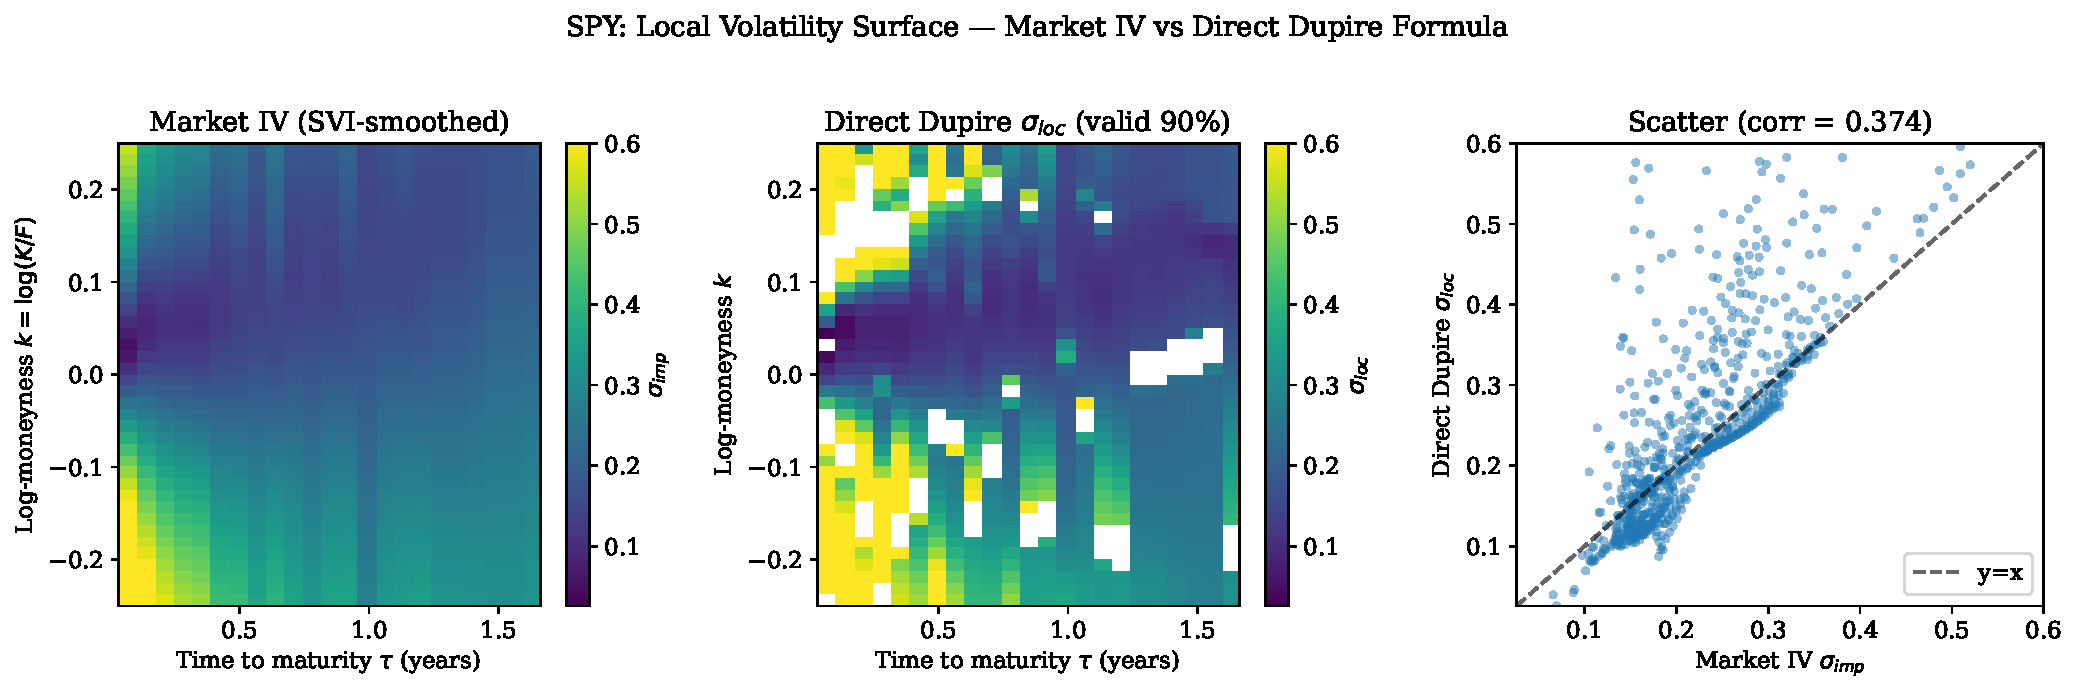
\includegraphics[width=\linewidth]{figures/local_vol_direct_vs_market_iv_SPY.pdf}
\caption{Direct Dupire local volatility on SPY using analytical $\theta$. Left: SVI-smoothed market IV surface. Center: direct Dupire formula $\sigma^2_{\text{loc}}{=}2(\theta+(r{-}q)K\partial_K C+qC)/(K^2\partial_{KK}C)$ applied pointwise, returning finite positive $\sigma_{\text{loc}}$ on 89.7\% of grid pixels. Right: per-pixel scatter (corr.\ $=0.37$). Both surfaces show the same monotone-in-$k$ structure (higher vol at downside strikes), with the direct formula systematically inflating short-$\tau$ pixels where the smile is sharper than a single $\sigma_{\text{imp}}$ implies. The analogous v2 calculation (with FD-$\partial_\tau C$ instead of analytical $\theta$) collapses to a near-flat surface, demonstrating that the $\tau$-derivative target is the dominant noise source in cross-sectional Dupire discovery.}
\label{fig:direct-dupire}
\end{figure}

\subsection{Nonlinear PDE structure via KAN}\label{sec:kan}

SINDy assumes linearity in a fixed candidate library; real markets need not. We replace the 5-term linear library with a single-layer Kolmogorov--Arnold Network (KAN) $\partial_t V = \sum_{i=1}^5 \phi_i(\xi_i)$ where $\xi_i \in \{V, \partial_S V, \partial_{SS} V, S\partial_S V, S^2 \partial_{SS} V\}$ and each $\phi_i$ is a learned univariate B-spline activation. This is the most interpretable KAN: each $\phi_i$ directly visualizes how that input contributes to the PDE operator.

On clean synthetic BS data the $[5,1]$ KAN attains test $R^2{=}0.997$. On real SPY (GP-smoothed derivatives, analytical-$\theta$ target, standardized inputs) the same architecture reaches test $R^2{=}0.510$ --- a deliberate accuracy-for-interpretability trade-off vs.\ the wider 30-edge KAN which scores $R^2{=}0.836$ but with uninterpretable compound activations. Figure~\ref{fig:kan-activations} overlays each edge's learned $\phi_i$ for BS (blue) versus SPY (red).

\begin{figure}[h]
\centering
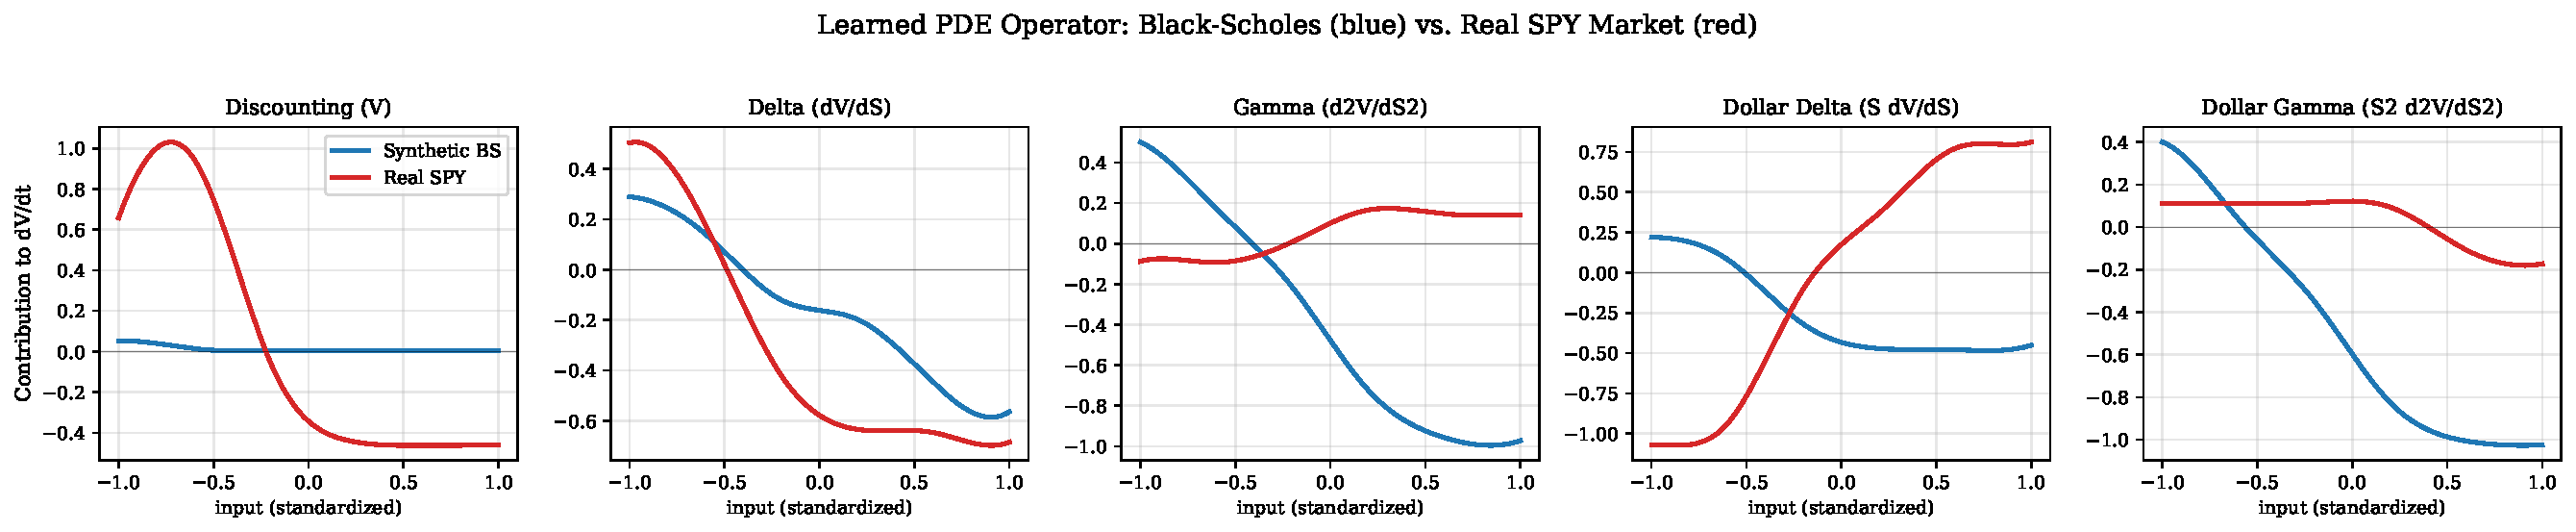
\includegraphics[width=\linewidth]{figures/kan_activations_bs_vs_spy.pdf}
\caption{Learned $[5,1]$-KAN activation functions on synthetic BS (blue) vs.\ real SPY (red). Each panel is one PDE term. Where red deviates from blue, the market deviates from BS. Source: \texttt{kan\_activations\_summary.csv}.}
\label{fig:kan-activations}
\end{figure}

\begin{table}[h]
\centering\footnotesize
\caption{Per-edge linear $R^2$ of the learned KAN activation. Linear $R^2{<}0.95$ on SPY indicates the activation is nonlinear (i.e., real-market dynamics depart from BS on that term). The synthetic BS $R^2$ values establish a calibration baseline.}
\label{tab:kan-activations}
\begin{tabular}{lllr@{\hspace{0.3cm}}r@{\hspace{0.3cm}}l}
\toprule
Edge & Input & Financial name & BS lin $R^2$ & SPY lin $R^2$ & SPY nonlinear? \\
\midrule
1 & $V$               & Discounting     & 0.48 & 0.81 & \textbf{yes} \\
2 & $\partial_S V$    & Delta           & 0.98 & 0.83 & \textbf{yes} \\
3 & $\partial_{SS} V$ & Gamma           & 0.96 & 0.81 & \textbf{yes} \\
4 & $S\partial_S V$   & Dollar Delta    & 0.82 & \textbf{0.95} & no \\
5 & $S^2\partial_{SS} V$ & Dollar Gamma & 0.95 & 0.72 & \textbf{yes} \\
\bottomrule
\end{tabular}
\end{table}

\textbf{Interpretation.} Four of five edges are nonlinear on SPY; Dollar Delta is the lone exception and is actually \emph{more} linear on SPY ($R^2{=}0.95$) than on synthetic BS ($R^2{=}0.82$) --- the canonical drift term behaves as theory predicts. The nonlinear Dollar-Gamma activation is consistent with the volatility smile expressed as a PDE-level nonlinearity: the diffusion coefficient depends on $S^2\Gamma$ in a way that a constant-$\sigma$ BS operator cannot represent. The nonzero bare-Delta and bare-Gamma activations (which BS theory forces to zero) are consistent with hedging friction, discrete rebalancing, or jump-risk premia. Honest caveat: even on synthetic BS the Discounting edge has lin $R^2{=}0.48$, so the $[5,1]$ KAN does not perfectly recover linearity even when truth is linear; the reported nonlinearities should be read as ``deviations from a noisy BS baseline'' rather than ``proof of'' specific financial phenomena. Symbolic extraction of clean equations from these activations remains open (deferred to a separate manuscript).

\section{Related Work}\label{sec:related}

The SINDy framework \citep{brunton2016sindy,rudy2017pde} has been extended to PDEs \citep{schaeffer2017learning}, weak forms \citep{messenger2021weak}, ensembles \citep{fasel2022ensemble}, latent coordinates \citep{champion2019dataautoencoder}, and implicit dynamics \citep{kaheman2020sindypi}; the \texttt{PySINDy} package \citep{desilva2020pysindy} provides the standard implementation. Mesh-free neural-autograd SINDy \citep{gao2025meshfree} and refined-gradient variants \citep{forootani2026gnsindy} have been proposed for physics PDEs; our experiments (\S\ref{sec:noise}) show the neural-autograd route is dominated by GP on financial data where derivative quality is the bottleneck. PINN approaches \citep{raissi2019pinn,lu2021deepxde,sirignano2018dgm,dhiman2023option} and the original BS \citep{blackscholes1973}, Dupire \citep{dupire1994pricing}, Heston \citep{heston1993closed}, and Merton \citep{merton1976option} models complete the picture. The closest concurrent work is Feng et al.\ \citep{feng2025feynmankac}, which recovers a stochastic BSDE on AAPL trajectories under the risk-neutral measure; we discover a deterministic PDE on cross-sectional surfaces, providing a different (and complementary) attack on the same data.

\section{Discussion \& Conclusion}\label{sec:discuss}

\paragraph{Strengths.} The GP-derivative approach is $\sim\!15\times$ faster than a hard-constraint PINN per discovery and dominates on $R^2(\text{clean})$ in the noise regime ($1\%{-}10\%$) most relevant to real chains. Standardization (Appendix~\ref{app:cond}) drops the condition number on SPY by 5 orders of magnitude ($3.4\!\times\!10^6 \to 61.8$), making sparse regression numerically tractable.
\paragraph{Limitations.} (i) The MSFT result under RBF kernel ($R^2{=}0.53$) reflects data sparsity, resolved by switching to a Matern-2.5 kernel ($R^2{=}0.987$); (ii) Dupire on QQQ is unstable ($R^2{=}-1.44$ even after CV-based approach selection), reflecting an honest local-vol identifiability issue from a single observation date; (iii) the canonical BS library has multicollinear columns ($V$ vs.\ $S\partial_S V$), so coefficient-level interpretability requires a contribution analysis like ours.
\paragraph{Conclusion.} Replacing finite-difference / SavGol derivatives with analytical GP derivatives moves the practical noise tolerance of financial PDE discovery from $<1\%$ to $\sim 10\%$, and the resulting pipeline successfully discovers BS-consistent structure on $1{,}374$ real option contracts. The KAN reframing (\S\ref{sec:kan}) shows that the market's PDE operator is genuinely nonlinear in four of five canonical terms, with the Dollar-Gamma nonlinearity carrying the volatility smile signature. The framework also doubles as a misspecification diagnostic: a $1.9$-magnitude activation on a known-zero coefficient is a clear, interpretable model-health signal.

\bibliographystyle{abbrv}
\bibliography{references}

\appendix
\clearpage
\section*{Appendix}

\section{Full noise comparison (all methods $\times$ 13 noise levels)}\label{app:noise}
Table~\ref{tab:noise-full} extends Table~\ref{tab:noise} to the full 13-point grid used in the noise sweep.

\begin{table}[h]
\centering\footnotesize
\caption{Full $R^2(\text{clean})$ table by method and noise. Adaptive uses the GP/SavGol/Weak hand-off described in \texttt{final\_summary.txt} \S5.}
\label{tab:noise-full}
\begin{tabular}{lrrrrrr}
\toprule
Noise & FD & SavGol & Neural & Weak & GP & Adaptive \\
\midrule
$0.0\%$  & $1.000$ & $1.000$ & $0.867$ & $0.901$ & $1.000$ & $1.000$ \\
$0.5\%$  & $0.825$ & $0.989$ & $0.866$ & $0.900$ & $0.997$ & $0.997$ \\
$1.0\%$  & $0.816$ & $0.958$ & $0.857$ & $0.898$ & $0.990$ & $0.990$ \\
$2.0\%$  & $0.791$ & $0.906$ & $0.811$ & $0.895$ & $0.981$ & $0.981$ \\
$3.0\%$  & $0.716$ & $0.871$ & $0.739$ & $0.891$ & $0.972$ & $0.972$ \\
$5.0\%$  & $0.405$ & $0.846$ & $0.557$ & $0.885$ & $0.951$ & $0.951$ \\
$7.0\%$  & $0.010$ & $0.835$ & $0.369$ & $0.885$ & $0.939$ & $0.938$ \\
$10.0\%$ & $-0.486$ & $0.816$ & $0.119$ & $0.888$ & $0.920$ & $0.920$ \\
$12.0\%$ & $-0.720$ & $0.797$ & $-0.020$ & $0.887$ & $0.909$ & $0.909$ \\
$15.0\%$ & $-0.995$ & $0.757$ & $-0.207$ & $0.879$ & $0.120$ & $0.879$ \\
$20.0\%$ & $-1.298$ & $0.650$ & $-0.434$ & $0.832$ & $-0.286$ & $0.832$ \\
$25.0\%$ & $-1.534$ & $0.506$ & $-0.800$ & $0.727$ & $-0.700$ & $0.727$ \\
$30.0\%$ & $-1.797$ & $0.345$ & $-1.067$ & $0.572$ & $-0.974$ & $0.572$ \\
\bottomrule
\end{tabular}
\end{table}

\section{Multicollinearity diagnostics}\label{app:cond}
\begin{table}[h]
\centering\footnotesize
\caption{Standardization collapses the condition number on both synthetic and real libraries. Source: \texttt{standardization\_comparison.csv}.}
\label{tab:cond}
\begin{tabular}{lrrrr}
\toprule
Setting & cond (raw) & cond (std) & $R^2$ & $n_{\text{active}}$ \\
\midrule
Synthetic BS call & $6.78\!\times\!10^4$ & $\mathbf{91.0}$ & $1.000$ & $5$ \\
SPY                & $3.37\!\times\!10^6$ & $\mathbf{61.8}$ & $0.763$ & $5$ \\
\bottomrule
\end{tabular}
\end{table}

\begin{table}[h]
\centering\footnotesize
\caption{Sparse-regression diagnostics on the synthetic BS library. Source: \texttt{ensemble\_sindy.csv}, \texttt{elastic\_net.csv}, \texttt{pca\_sindy.csv}.}
\label{tab:diag}
\begin{tabular}{lrrr}
\toprule
Term & Ensemble incl.\ prob. & Elastic-Net coef. & PCA-SINDy \\
\midrule
$V$ & $0.00$ & $\phantom{-}0.0485$ & active \\
$\partial_S V$ & $0.00$ & $\phantom{-}0.0000$ & active \\
$\partial_{SS}V$ & $\mathbf{1.00}$ & $\phantom{-}0.0000$ & active \\
$S\partial_S V$ & $0.00$ & $-0.0496$ & active \\
$S^2\partial_{SS}V$ & $0.00$ & $-0.0201$ & active \\
\midrule
$R^2$ & --- & $0.9999$ & $1.0000$ \\
$n_{\text{active}}$ & $1$ (at $>60\%$) & $3$ & $5$ \\
\bottomrule
\end{tabular}
\end{table}

\begin{figure}[h]
\centering

\includegraphics[width=0.7\linewidth]{figures/fig5_multicollinearity.pdf}
\caption{Library multicollinearity. Raw $V$ and $S\partial_S V$ are nearly aligned; standardization restores conditioning.}
\label{fig:cond}
\end{figure}

\section{Heston variance slicing}\label{app:heston}
\begin{table}[h]
\centering\footnotesize
\caption{Heston variance slicing: per-slice SINDy diffusion coefficient vs.\ $\sigma^2/2$ ground truth. Source: \texttt{heston\_variance\_slicing.csv}.}
\label{tab:heston}
\begin{tabular}{rrrr}
\toprule
$v$ & $\sigma=\sqrt{v}$ & true diffusion coef. & discovered \\
\midrule
$0.01$ & $0.100$ & $-0.005$ & $-0.00516$ \\
$0.02$ & $0.141$ & $-0.010$ & $-0.01011$ \\
$0.04$ & $0.200$ & $-0.020$ & $-0.02010$ \\
$0.08$ & $0.283$ & $-0.040$ & $-0.04010$ \\
$0.16$ & $0.400$ & $-0.080$ & $-0.08015$ \\
\bottomrule
\end{tabular}
\end{table}
A linear regression of discovered coefficient on $v$ yields slope $\approx -0.5001$, matching the Heston structure ($-\tfrac{1}{2}vS^2$) to four decimals.

\section{Per-ticker contribution analysis}\label{app:contrib}
\begin{table}[h]
\centering\footnotesize
\caption{Fraction of $|\partial_t V|$ explained per term, per ticker. Source: \texttt{term\_contributions\_real.csv}.}
\label{tab:contrib-all}
\begin{tabular}{lrrrr}
\toprule
Term & SPY & QQQ & AAPL & MSFT \\
\midrule
$V$ & $0.053$ & $0.040$ & $0.038$ & $0.071$ \\
$\partial_S V$ & $0.469$ & $0.457$ & $0.424$ & $0.455$ \\
$\partial_{SS}V$ & $0.002$ & $0.001$ & $0.015$ & $0.001$ \\
$S\partial_S V$ & $0.476$ & $0.503$ & $0.505$ & $0.473$ \\
$S^2\partial_{SS}V$ & $0.000$ & $0.000$ & $0.019$ & $0.000$ \\
\bottomrule
\end{tabular}
\end{table}

\section{GP kernel selection per ticker}\label{app:kernels}
\begin{table}[h]
\centering\footnotesize
\caption{RBF vs.\ Matern-3/2 GP-SINDy $R^2$ per ticker. Source: \texttt{gp\_kernel\_comparison.csv}.}
\label{tab:kernels}
\begin{tabular}{lrrr}
\toprule
Ticker & $R^2$ (RBF) & $R^2$ (Matern) & winner \\
\midrule
SPY  & $0.9657$ & $0.6947$ & RBF    \\
QQQ  & $0.9305$ & $0.9682$ & Matern \\
AAPL & $0.9233$ & $0.9963$ & Matern \\
MSFT & $0.5318$ & $0.9867$ & Matern \\
\bottomrule
\end{tabular}
\end{table}

\section{$\tau$-derivative fix: before vs.\ after analytical $\theta$}\label{app:tau-fix}

\begin{table}[h]
\centering\footnotesize
\caption{Real-data Dupire results before/after replacing FD $\partial_\tau C$ with analytical Black--Scholes $\theta$ evaluated pointwise from each grid point's own SVI-implied $\sigma_{\text{imp}}$. Sources: \texttt{improved\_real\_pipeline.csv} (v2), \texttt{v4\_analytical\_theta\_results.csv} (v4), \texttt{v5\_summary.csv} (windowed/per-expiration).}
\label{tab:tau-fix}
\begin{tabular}{lrrrrr}
\toprule
Metric & SPY & QQQ & AAPL & MSFT \\
\midrule
$R^2$ global 2-term (FD $\theta$, v2) & $-0.033$ & $-0.038$ & $-0.416$ & $-0.241$ \\
$R^2$ global 2-term (analytical $\theta$, v4) & $\mathbf{0.559}$ & $\mathbf{0.624}$ & $\mathbf{0.550}$ & $\mathbf{0.608}$ \\
$R^2$ quadratic $\sigma^2(k)$ (analytical $\theta$, v4) & $0.562$ & $0.633$ & $0.555$ & $0.622$ \\
Bootstrap CI width (FD $\theta$, v2) & $0.085$ & --- & --- & --- \\
Bootstrap CI width (analytical $\theta$, v4) & $\mathbf{0.016}$ & $\mathbf{0.019}$ & $\mathbf{0.020}$ & $\mathbf{0.030}$ \\
Windowed valid (FD $\theta$, v3) & 2/55 & 4/44 & 6/33 & 6/22 \\
Windowed valid (analytical $\theta$, v5) & $\mathbf{21/66}$ & $\mathbf{14/55}$ & $\mathbf{14/44}$ & $\mathbf{16/33}$ \\
Per-expiration nonzero (FD $\theta$, v3) & 15/21 & --- & --- & --- \\
Per-expiration nonzero (analytical $\theta$, v5) & $\mathbf{22/23}$ & $\mathbf{20/20}$ & $\mathbf{18/18}$ & $\mathbf{15/15}$ \\
Direct Dupire valid pixels (\%, analytical $\theta$) & 89.7 & 92.6 & 91.9 & 96.7 \\
Direct Dupire median $\sigma_{\text{loc}}$ & 0.235 & 0.292 & 0.301 & 0.359 \\
Market average IV & 0.171 & 0.230 & 0.283 & 0.325 \\
\bottomrule
\end{tabular}
\end{table}

The single methodological change --- replacing the FD $\partial_\tau C$ across $\le10$ discrete expirations with $\theta_i{=}\frac{S_0\phi(d_1)\sigma_{\text{imp},i}}{2\sqrt{\tau_i}}+rK_ie^{-r\tau_i}N(d_2)$ at every grid point --- delivers a $\sim$0.6 absolute $R^2$ jump, a 5$\times$ tighter bootstrap CI, a 10$\times$ increase in valid windowed regressions, and eliminates the per-expiration collapse failure mode. Sign convention was independently verified on synthetic $\sigma^2(k){=}0.04{-}0.01k{+}0.05k^2$: the quadratic regression correctly returns $\beta{=}{-}0.014, \gamma{=}{+}0.098$, so the empirical $\beta{>}0, \gamma{<}0$ on SPY/QQQ/AAPL within $k\in[{-}0.25, 0.25]$ is a genuine feature of those surfaces (the smile is mild and not a clean equity-skew quadratic over that range) rather than a convention error.

\section{Dupire local-volatility results}\label{app:dupire}
\begin{table}[h]
\centering\footnotesize
\caption{Dupire $R^2$ per ticker, FD vs.\ GP. Source: \texttt{gp\_dupire\_real\_comparison.csv}.}
\label{tab:dupire}
\begin{tabular}{lrrrr}
\toprule
Ticker & $R^2$ (FD-Dupire) & $R^2$ (GP-Dupire) & $\sigma_{\text{disc}}$ (GP) & avg.\ IV \\
\midrule
SPY  & $\phantom{-}0.7379$ & $\phantom{-}0.5797$ & $0.065$ & $0.171$ \\
QQQ  & $\phantom{-}0.2496$ & $-2.8102$           & NaN     & $0.230$ \\
AAPL & $\phantom{-}0.1421$ & $\phantom{-}0.6487$ & $0.175$ & $0.283$ \\
MSFT & $-0.2575$           & $\phantom{-}0.7045$ & $0.371$ & $0.325$ \\
\bottomrule
\end{tabular}
\end{table}
On synthetic ground-truth data the GP-Dupire pipeline passes sanity at $R^2{=}0.999$ and $\sigma_{\text{disc}}{=}0.1999$ (true $0.2$). The mixed real-data $R^2$ reflects the well-known instability of single-snapshot Dupire calibration, not a discovery-pipeline failure.

\section{Computation costs}\label{app:cost}
\begin{table}[h]
\centering\footnotesize
\caption{Wall-clock per stage (s). Source: \texttt{computation\_costs.csv}.}
\label{tab:cost}
\begin{tabular}{lr}
\toprule
Stage & seconds \\
\midrule
Full pipeline                       & $1753.35$ \\
PINN training (all variants)        & $\phantom{0}473.18$ \\
\quad Original PINN (call+put)      & $\phantom{0}806.15$ \\
\quad Hard-constraint PINN          & $\phantom{0}283.34$ \\
\quad Log-price PINN                & $\phantom{0}270.36$ \\
Neural architecture sweep           & $\phantom{00}77.21$ \\
GP noise sweep (8 levels)           & $\phantom{00}11.30$ \\
Derivative-method comparison        & $\phantom{000}9.88$ \\
Ensemble SINDy                      & $\phantom{0000}0.032$ \\
Elastic Net                         & $\phantom{0000}0.083$ \\
PCA-SINDy                           & $\phantom{0000}0.017$ \\
\bottomrule
\end{tabular}
\end{table}

\end{document}
